% !TeX root = ../main.tex

\chapter{模型结果}

\section{描述性统计分析}
\begin{table}[H]
  \centering
  \begin{minipage}{.45\linewidth}
    \centering
    \caption{收盘价描述性统计结果}
    \label{shoupan}
    \begin{tabular}{cl}
      \toprule
      收盘价   & 结果              \\
      \midrule
      平均值 & \num{0.06282988}        \\
      标准差 & \num{0.01003973}        \\
      最小值 & \num{0.04486}           \\
      最大值 & \num{0.0842}            \\
      中位数 & \num{0.0611}            \\
      \bottomrule
    \end{tabular}
  \end{minipage}%
  \hspace{0.05\linewidth}
  \begin{minipage}{.45\linewidth}
    \centering
    \caption{收盘价日变化描述性统计结果}
    \label{bianhua}
    \begin{tabular}{cl}
      \toprule
      日变化   & 结果              \\
      \midrule
      平均变化 & \num{-7.039262e-05}     \\
      标准差 & \num{0.006726684}       \\
      最小变化 & \num{-0.0886}           \\
      最大变化 & \num{0.0985}            \\
      中位数 & \num{0}                 \\
      \bottomrule
    \end{tabular}
  \end{minipage}
\end{table}

\section{时间序列分析}
\subsection{移动平均}
\begin{figure}[H]
  \centering
  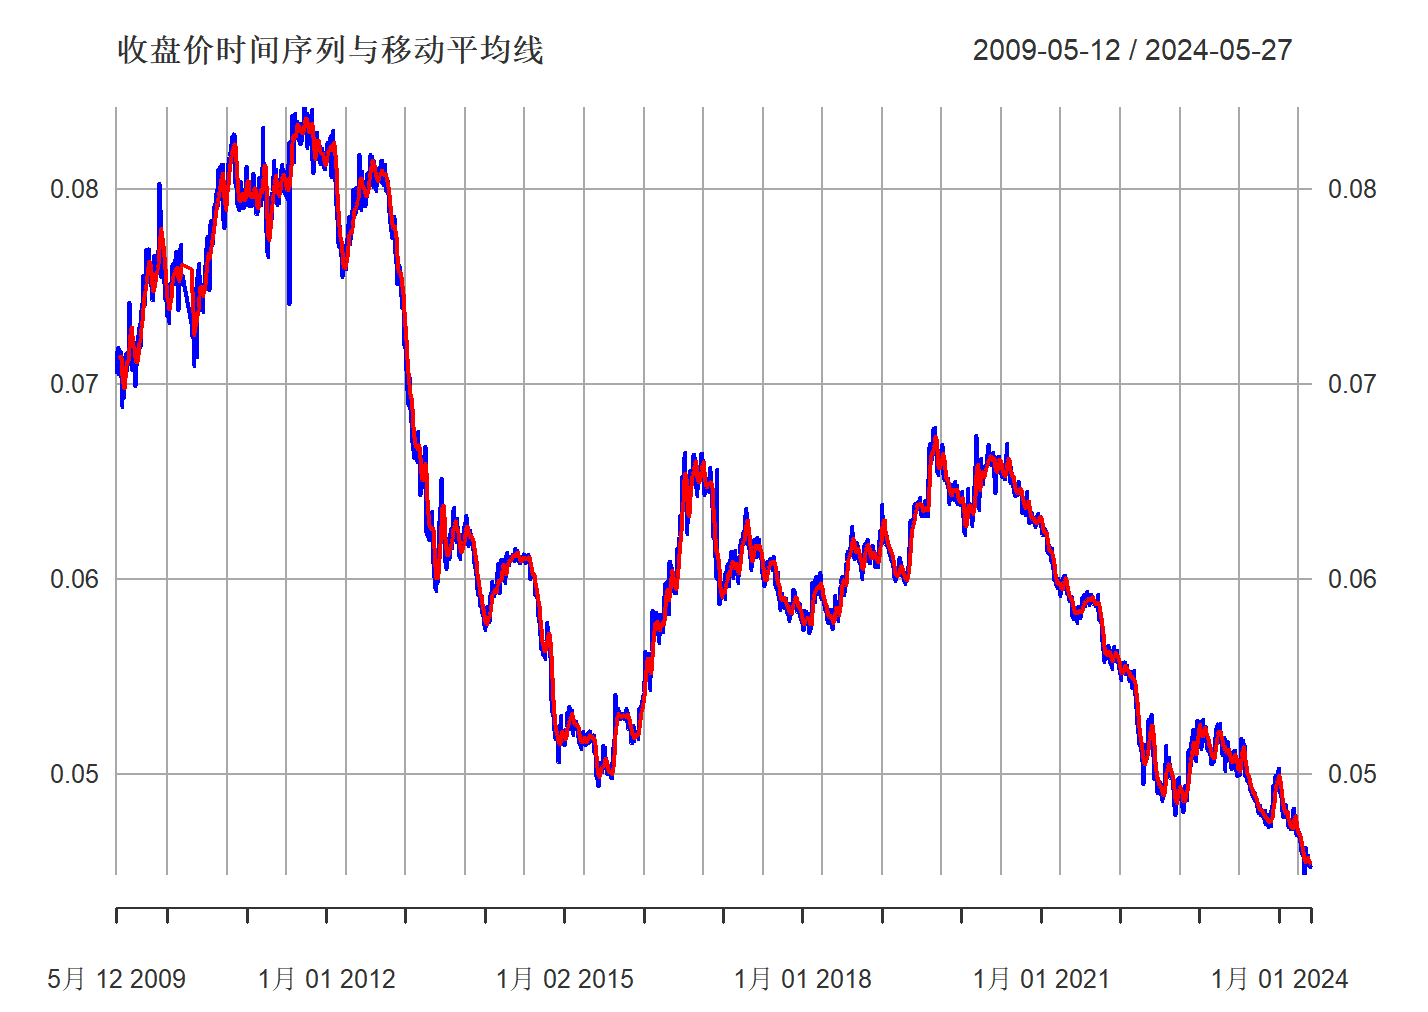
\includegraphics[width=\textwidth]{shoupanjia.png}
  \caption{收盘价时间序列与移动平均线}
  \label{shijian}
  \note{注:图中蓝色线为收盘价时间序列线;红色线为移动平均线。}
\end{figure}
\subsection{ARIMA模型}
\begin{figure}[H]
  \centering
  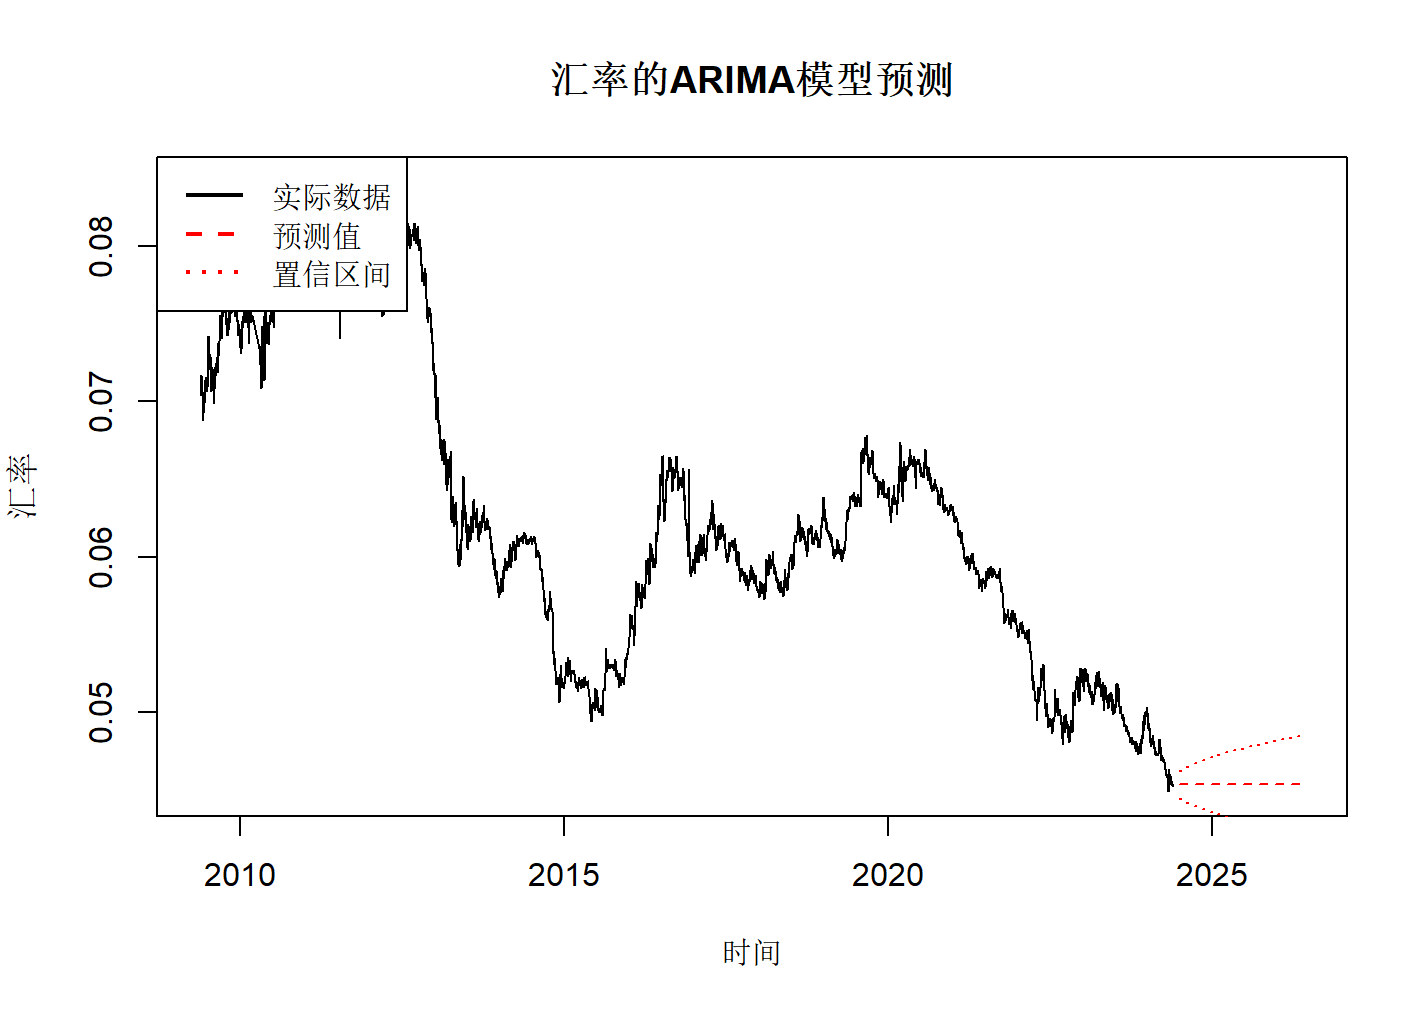
\includegraphics[width=0.91\textwidth]{ARIMA.png}
  \caption{汇率的ARIMA模型预测}
  \label{ARIMA}
\end{figure}

\section{波动性分析}
\subsection{GARCH模型}
\begin{figure}[H]
  \centering
  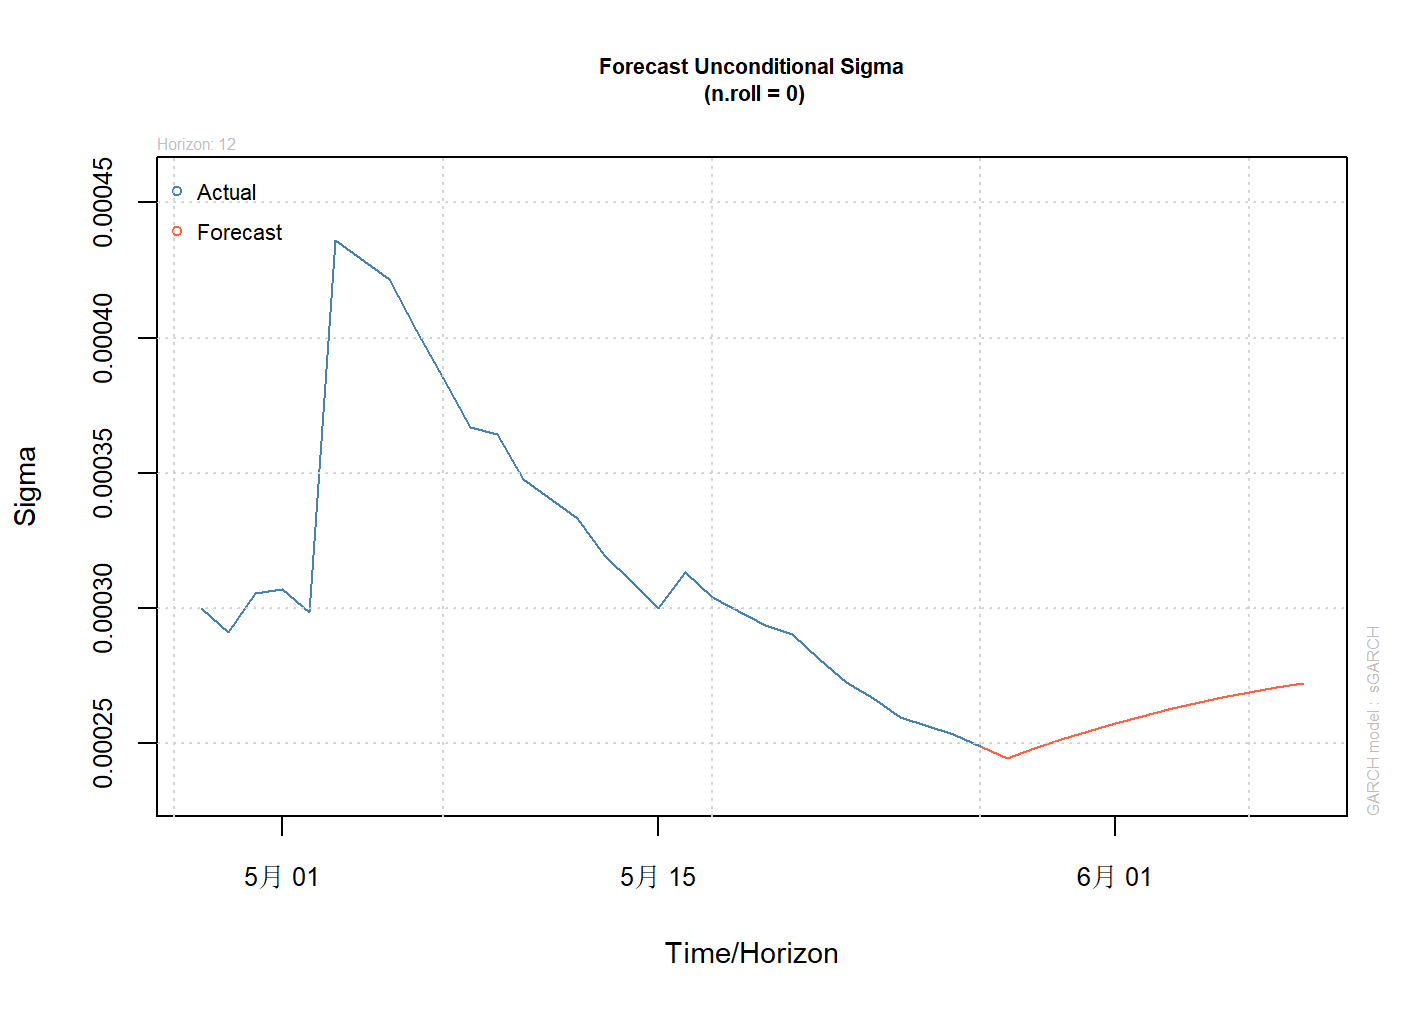
\includegraphics[width=0.91\textwidth]{GARCH.png}
  \caption{汇率的GARCH模型预测}
  \label{GARCH}
\end{figure}
\subsection{EGARCH模型}
\begin{figure}[H]
  \centering
  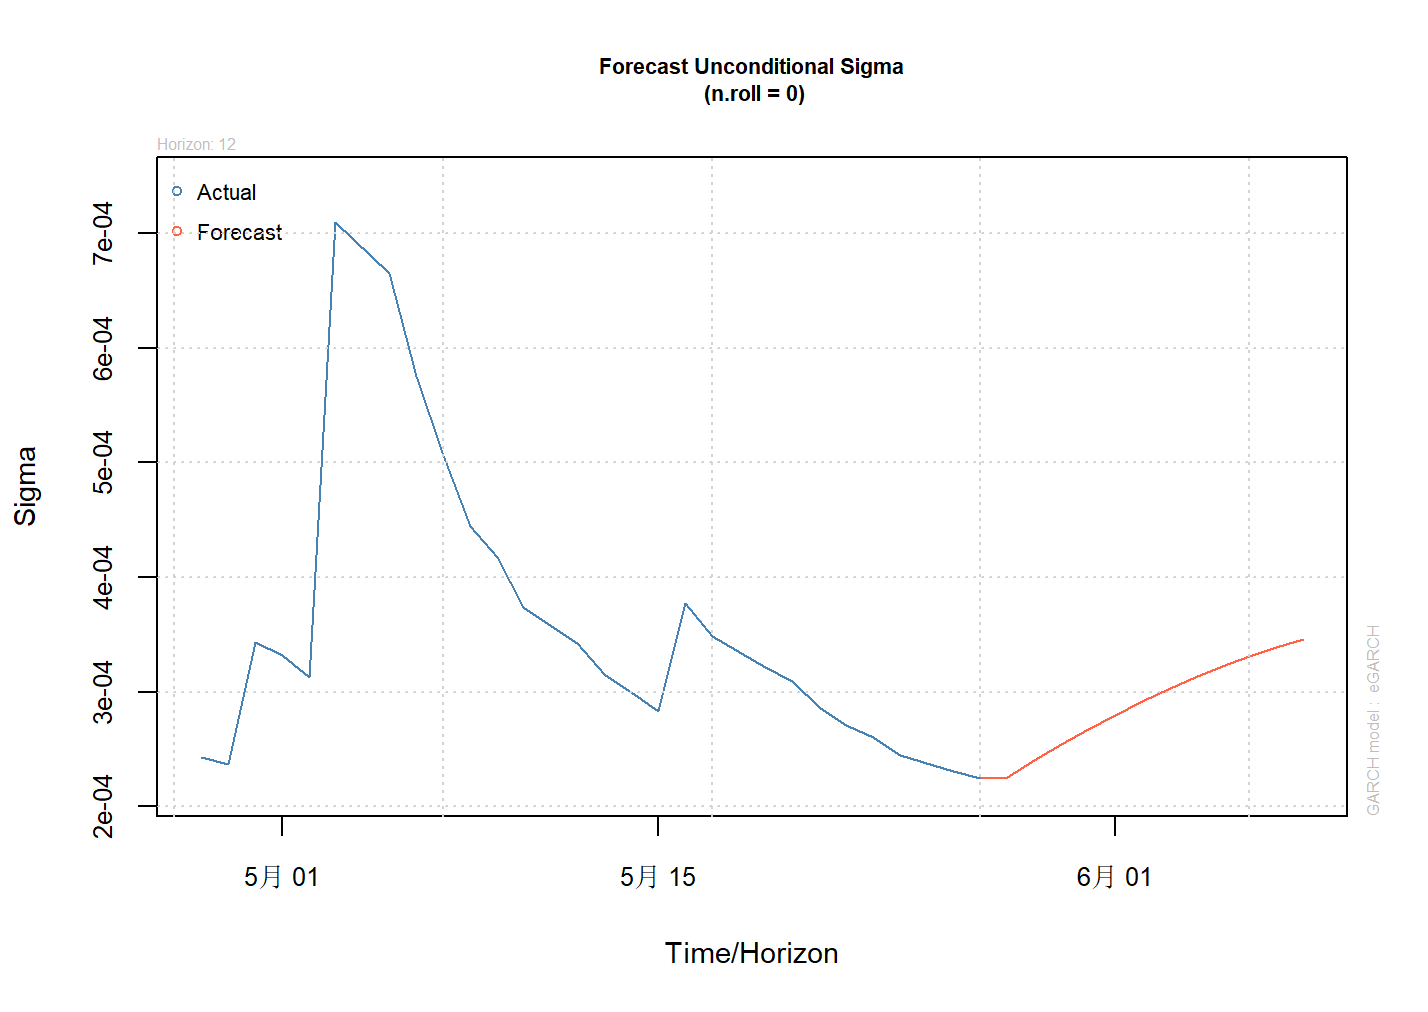
\includegraphics[width=\textwidth]{EGARCH.png}
  \caption{沪铝的EGARCH模型预测}
  \label{EGARCH}
\end{figure}

\section{风险分析}
\subsection{VaR分析}
\begin{table}[H]
  \centering
  \caption{VaR分析结果}
  \label{VaR}
  \begin{tabular}{cl}
    \toprule
    类型   & 结果                                       \\
    \midrule
    VaR & \num{-0.009756969}\\
    \bottomrule
  \end{tabular}
\end{table}

\subsection{情景分析和压力测试}
\begin{table}[H]
  \centering
  \caption{情景分析和压力测试结果}
  \label{qingjing}
  \begin{tabular}{cl}
    \toprule
    类型   & 结果                                       \\
    \midrule
    VaR & \num{-0.05975697}\\
    \bottomrule
  \end{tabular}
\end{table}